\section{Server subsystems analysis}

The OCP has defined a specification for a server that can be used in a DC. This is the Decathlete specification. Intel, based on the Decathlete specification, has created the Intel S2600GZ server. Therefore, in this thesis, the server that is being used is an Intel S2600GZ server. \cite{serverSpecif} \cite{serverGuide}

\begin{figure}[H]
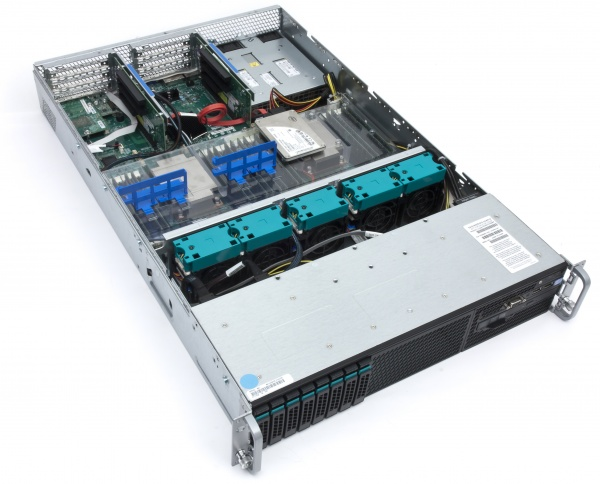
\includegraphics[scale= 0.5]{intel-r2000-s2600gz-server} % Podría poner[width=\linewidth]
\caption{Intel s2600GZ server.}
\label{fig:decathlete} %Establece una etiqueta para la figura
\end{figure}

Next, a brief information about the CPU, Fans, Hard drives and Memories will be explained in order to establish the scenario in which the thesis will developed. For each subsystem we will analyze the impact on overall power consumption and the control knobs available.

The hardware configuration of the Decathlete server in the Green LSI is not completely full. The number of components supported and those mounted in the server are detailed in Table \ref{tab:components}.

\begin{table}[H]
\begin{center}
\begin{tabular}{p{6cm} p{3cm} p{3cm}}
  \hline
  %\multicolumn{2}{c}{Components supported by the server}
  Components & Supported & Green LSI \\
  \hline
  Number of processors & 2 & 1 \\
  Number of DIMMS & 24 & 8 \\
  Number of Fans & 5 & 5 \\
  Number of power sources & 2 & 2 \\
  \hline
\end{tabular}
\end{center}
\caption{Components of the Green LSI s2600GZ server.}
\label{tab:components}
\end{table}

Therefore  according to previous work in the Green LSI team, the major part of the consumption comes from four contributors, the total consumption of the server can be divided into the following components:

\begin{equation*}
P_{TOTAL} = P_{CPU} + P_{MEMS} + P_{FANS} + P_{DISKS} + P_{OTHERS}
\end{equation*}

Where each of the terms are the power consumption of each of most important contributors to the total amount and OTHERS brings together the consumption of the rest of the components of the server - i.e.service processor, sensors, BMC, etc. - whose contributions can be considered negligible.

\begin{wrapfigure}{l}{0.5\textwidth}
    \centering
    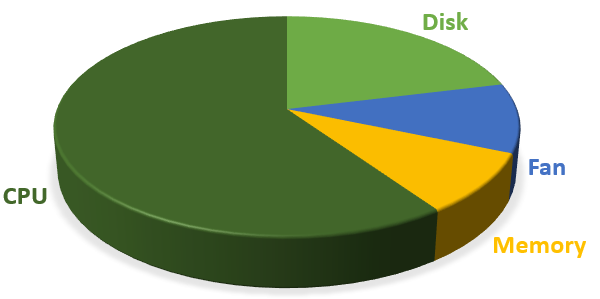
\includegraphics[width=0.5\textwidth]{totCons2}
    \caption{Average Decathlete's power consumption breakdown}
    \label{fig:totCons} %Establece una etiqueta para la figura
\end{wrapfigure}

Figure \ref{fig:totCons}~represents the breakdown of the main power consumption contributors of the server

This is the reason why the key data of their consumption will be studied down below.


\ \\ \ \\ \ \\ \ \\ \ \\
    \subsection{CPU}
    
    
    
    
    The Intel S2600GZ processor is an Intel® Xeon® Processor E5-2620 \cite{procDatasheet1} \cite{procDatasheet2} which has the specifications of Table \ref{tab:cpu_spec}.
    
\begin{table}[H]
\begin{center}
\begin{tabular}{p{6cm} p{3cm}}
  \hline
  \bf Number of cores & 6 \\
  \bf Number of threads & 12  \\
  \bf Processor base frequency & 2 GHz  \\
  \bf Range of scaling frequencies & 1.2 - 2.0 GHz. \\
  \bf Power & 85 W \\
  \hline
\end{tabular}
\end{center}
\caption{Specifications of the Intel® Xeon® Processor E5-2620. \cite{procTabla}}
\label{tab:cpu_spec}
\end{table}
%http://www.intel.com/content/www/us/en/processors/xeon/xeon-e5-brief.html

\begin{figure}[H]
\begin{center}
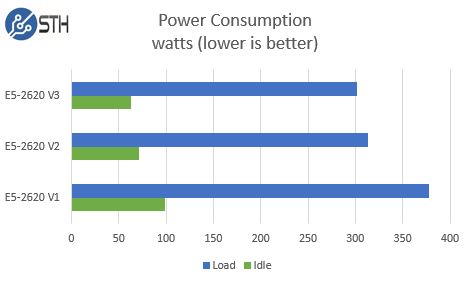
\includegraphics[scale= 1]{Intel-Xeon-E5-2620-V1-V2-V3-Power-Consumption} % Podría poner[width=\linewidth]
\caption{Power consumption of the Intel Processor \cite{procGrafica}}
\label{fig:Intel-Xeon-E5-2620-V1-V2-V3-Power-Consumption}
\end{center}
\end{figure}
%http://www.servethehome.com/dual-intel-xeon-e5-2620-v1-v2-v3-compared/

The breakdown of the power consumption of the CPU is the following:

\begin{equation*}
P_{CPU} = P_{CPU_{idle}} + P_{CPU_{leakage}} + P_{CPU_{dyn}} 
\end{equation*}
where:
\begin{itemize}
    \item[$-$] $P_{CPU_{idle}}$ is the consumption of the CPU when the server is not executing any load.
    \item[$-$] $P_{CPU_{leakage}}$ is the consumption associated with the leakage current in the CMOS. This consumption is exponential with the temperature.
    \item[$-$] $P_{CPU_{dyn}}$ is the consumption associated with the execution of the workload.
\end{itemize}


In this thesis, two actuation techniques associated with the processor will be checked.

\subsubsection{DVFS}

Dynamic Voltage and Frequency Scaling is a framework to change the frequency and/or operating voltage of a processor(s) based on system performance requirements at the given point of time.

Voltage scaling is achieved using voltage layer and regulator framework(driver). When frequency is scaled, voltage corresponding to the frequency is looked-up in the opp list. The device scale function requires the voltage layer to scale the device voltage to the target voltage.

The consumption saving is due to the switching power dissipated by a chip using static CMOS gates is 

\begin{equation*}
C * {V}^{2} * f
\end{equation*}
where:
\begin{itemize}
    \item[$-$] C is the capacitance being switched per clock cycle,
    \item[$-$] V is the supply voltage,
    \item[$-$] f is the switching frequency
\end{itemize}

so this part of the power consumption decreases quadratically with voltage. The formula is not exact however, as many modern chips are not implemented using 100$\%$ CMOS, but also use special memory circuits, dynamic logic such as domino logic, etc. Moreover, there is also a static leakage current, which has become more and more accentuated as feature sizes have become smaller (below 90 nanometres) and threshold levels lower.

\subsubsection{Turning ON-OFF CPUs}

Another technique that has been introduced in current servers and desktop computers is, when there are several CPUs, turning off some. This is necessary when the workload is too low or it cannot be spread into several cores.
%Esto ya se hace a nivel de BIOS

The idea is that, despite the CPU is not been used, power consumption due to leakage power is still there. This consumption emanates at a micro-level in transistors. Small amounts of currents are always flowing between the differently doped parts of the transistor. The magnitude of these currents depend on the state of the transistor, its dimensions, physical properties and sometimes temperature. The total amount of leakage currents tends to inflate for increasing temperature and decreasing transistor sizes.

This contribution is not as important as others, but it is easier to implement. In fact, there are some current policies based on this technique in the newest processors of the market. 

%%NO ES LO MISMO DISABLING QUE TURNING OFF

In this thesis, the idea has been disabling some CPU threads in order to study if the minimization of the power consumption balances out with the reduction of the computing power. This point will be developed in the next chapter.
%Insertar tabla






    \subsection{Fans}
    
    The server uses five fans of the company Nidec Corporation. The current configuration of the servers makes impossible to turn off one of the fans so they consume, according to the datasheet, 3.84 (W) per fan when they are at 4500 RPM. As there are five fans, the totally of fans consume 19.2 (W).
    
    \begin{comment}
    Additionally, related to the revolutions per minute (RPM) they can achieve, they have a maximum and a minimum cap:
    
\begin{itemize}
    \item[$-$] All the fans have a minimum RPM which is 6000 RPM. Regardless of the status of the server - idle, full-load, middle-load - fans cannot run at a lower speed.
    \item[$-$] The maximum speed that fans can achieve is 12.500 RPM which is an
    information obtained from the datasheet.
\end{itemize}
    \end{comment}


If any fan sensor or software detects that there is a failure or that there is not enough information to be sure that there is no failure, fans immediately start to run at full speed. Additionally, when one of the Hot-swap fans is removed to install another one, the time elapsed in which there are only four fans, they work at full speed, too.

\subsubsection{Reducing Fan speed}

%% Debería hablar de esto:
%%http://blog.stuffedcow.net/2012/10/intel32nm-22nm-core-i5-comparison/
%% Punto ideal de temperatura y consumo

Another way of reducing the energy consumption is reducing the air flow entered by the fans inside the server. According to the previous Green LSI study, DCs are over-refrigerated in some cases inducing a consumption expenditure that is not necessary.

The idea would be to study the impact of reducing the air flow - always being aware of compromise any server component. The consumption impact will depend on three variables: Density of the air, area of the fan and the air flow the fan moves.

According to this fact, the power consumed by a fan will respond as follows:
\begin{equation*}\label{eq:1}
Power\ = \frac{1}{2} * \rho * A * {V}^{3}
\end{equation*}
where:
\begin{itemize}
    \item[$-$] $\rho$ is the density of the air,
    \item[$-$] A is the area of the fan which is related to the size,
    \item[$-$] V is the air velocity
\end{itemize}

As the relation between energy and power is:
\begin{equation*}\label{eq:2}
Energy  = Power * Time
\end{equation*}

the relation between the air flow and the energy will be:
\begin{equation*}\label{eq:3}
Air\ flow\ \ \ \ is\ proportional\ to\ \ \ \ \ \sqrt[3] {Energy}
\end{equation*}

The conclusion is that this can be an important point to develop due to the fact that there is a chance that there is a considerable amount power saved. 

\begin{figure}[H]
\begin{center}
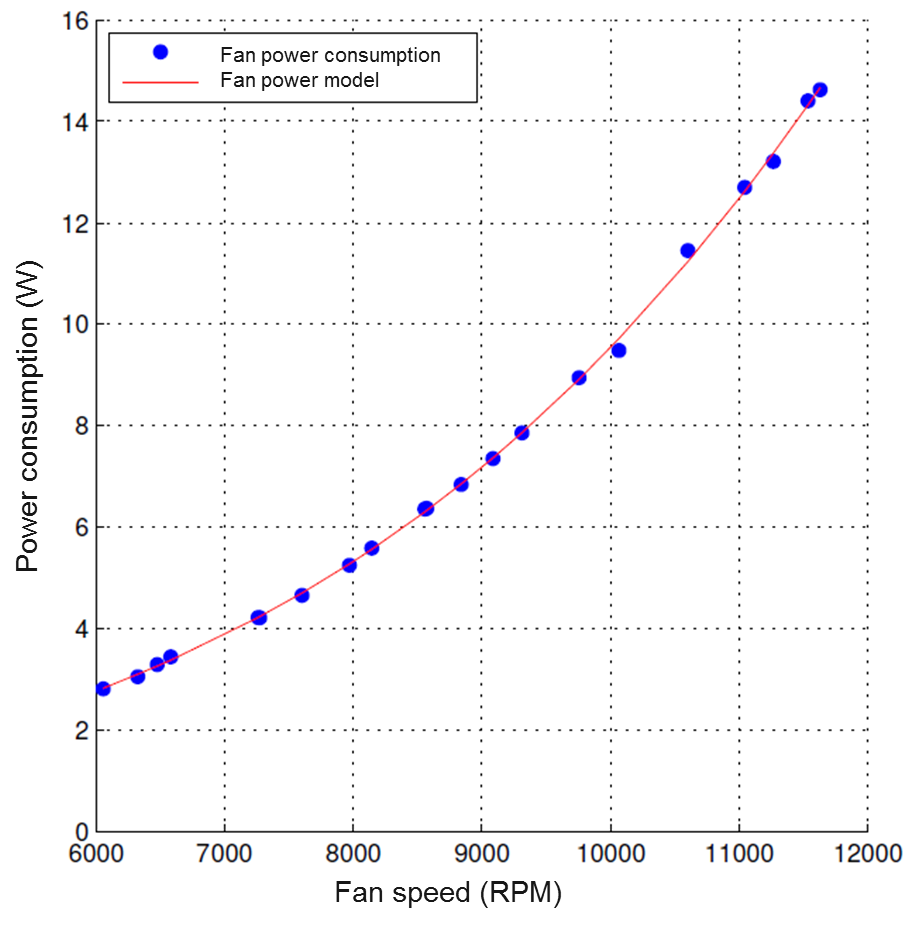
\includegraphics[scale= 0.7]{fan_speed3} % Podría poner[width=\linewidth]
\caption{Power spent depending of the RPM of the fan (~ Air Flow) in a generic server}
\label{fig:fan_speed} %Establece una etiqueta para la figura
\end{center}
\end{figure}
% Esto viene de https://www.usenix.org/legacy/event/hotpower08/tech/full_papers/tolia/tolia_html/index.html





    
    \subsection{Hard drives}
    
%http://www.seagate.com/www-content/product-content/constellation-fam/constellation/constellation-2/en-us/docs/constellation2-fips-ds1719-4-1207us.pdf

The server has four hard drives. The hard drives are designed by Seagate and the model is Constellation 2 \cite{diskDatasheet}. They have 1 TB of storage and use SAS as communication protocol.
    
\begin{table}[H]
\begin{center}
\begin{tabular}{p{8cm} p{3cm}}
  \hline
  \bf Idle power & 3.85 W \\
  \bf Typical Operating, Random Read & 6.4 W \\
  \bf Power Supply Requirements & +12V and +5V  \\
  \bf PowerChoice Technology & As low as 1.87 W  \\ 
  \hline
\end{tabular}
\end{center}
\caption{Specifications of the Seagate Constellation.2 SAS 1TB}
\label{tab:disk_spec}
\end{table}
    
Since there are used four hard drives, the consumption of the table has to be multiplied by four, remaining the total power consumption:
\begin{table}[H]
\begin{center}
\begin{tabular}{p{8cm} p{3cm}}
  \hline
  \bf Idle power & $3.85 * 4 = 15.4 W$ \\
  \bf Typical Operating, Random Read & $6.4 * 4 = 25.6 W$ \\
  \hline
\end{tabular}
\end{center}
\caption{RAID consumption Green LSI Decathlete}
\label{tab:disk_spec2}
\end{table}
    
    \subsection{Memory}
    
%% http://www.kingston.com/dataSheets/KVR16E11K4_32.pdf

Memories are from the model KVR16E11K4/32 from Kingston company \cite{memoryDatasheet}. In total, there are 32 GB of memory installed in the Decathlete, so there are eight modules of 4 GB each. The part of the information of the datasheet that is important for the thesis is the one presented in Table \ref{tab:mem_spec}

\begin{table}[H]
\begin{center}
\begin{tabular}{p{8cm} p{5cm}}
  \hline
  \bf Maximum Operating Power &  2.902 W (per module) \\
  \bf Total Maximum Operating Power & $2.902 * 8 = 23.21 W$ \\
  \hline
\end{tabular}
\end{center}
\caption{Memories consumption of the server}
\label{tab:mem_spec}
\end{table}

\subsubsection{Memories hotplugging}

Memories hotplugging is the same idea as turning on-off cpus. As it has been shown in the section above, memories consume around a quarter of all consumption of the server in idle status. This is the reason the memories have been selected to be studied.

Sometimes, the processes that are being executed in the server are not limited by the memories and they are being underused. In this cases, it would be interesting to shut down some memories so that server could save some energy.

This technique is not so widespread as turning off CPUs due to the fact that all the data allocated in that section of the memory must be moved to other section before turning the memory off. It is not so obvious to know exactly where the information is.

Due to the lack of an specific tool to perform this task, the procedure to achieve this goal will be detailed in Chapter 3.